\chapter{Computer Vision Solution For Collaborative
Pedestrian Indoor Navigation
}
 
%%%%%%%%%%%%%%%%%%%%%%%%%%%%%%%%%%%%%%%%%%%%%%%%%%%%%%%%%%%%
%%%%%%%%%%%%%%%%%%%%  NEW SECTION   %%%%%%%%%%%%%%%%%%%%%%%%
%%%%%%%%%%%%%%%%%%%%%%%%%%%%%%%%%%%%%%%%%%%%%%%%%%%%%%%%%%%%
\setcounter{equation}{0}
Cameras are used in pedestrian navigation for providing
velocity and heading information, and thus complementing
the conventional inertial sensors. While the inertial sensor
measurements suffer from drift, computer vision methods are
degraded by dynamic objects in the environment and lack of
features when the scene consists of surfaces with very uniform material. Unfortunately, the scenes in this collaborative
navigation consist of both; other members of this collaborative
team as dynamic objects and outdoor areas covered with snow
and feature poor office spaces indoors.\\
Traditionally monocular cameras have been used in pedes-
trian navigation due to their good performance combined
with small size. However, speed measurements suffer from
scale ambiguity due to the inability of monocular cameras
to measure the distance between objects and themselves.
Research has been active in solving the problem, but solutions
have often been suitable only for limited use cases. Recent
improvement in the quality of small RGB-D cameras provides good opportunities for computer vision based navigation
applications. RGB-D cameras, such as the RealSense product
family manufactured by Intel, provide the depth of tracked
objects and therefore solve the scale problem.\\
Depth camera measures the distance d between the camera’s
optical center and an object point \begin{math}X =(X, Y, Z )^T\end{math}.
When the camera is modeled as a pinhole camera we can get the real
3D coordinates of X using
\begin{center}
   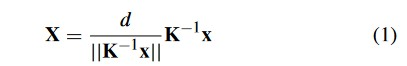
\includegraphics{eq1.jpg}
   \end{center}
  
where K is the calibration matrix including the camera intrinsics and x homogeneous image pixel coordinates
\begin{math}x = (x, y, 1)^T \end{math}. Rigid transformation of the point X from
the camera centered coordinate system to the arbitrary world
coordinate frame \begin{math}
X_w
\end{math} is defined by the rotation R and translation T of the camera with respect to the world frame as
\begin{center}
   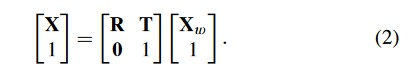
\includegraphics{eq2.jpg}
   \end{center}
When the authors are looking at the motion between two consecutive images they  get the real metric displacement of the camera by setting the origin to the first camera center
\begin{math}(T_1 = (0, 0, 0)^T )\end{math}, defining the coordinate axis being aligned
with the camera orientation \begin{math}(R_1 = I)\end{math}, where I is the identity
matrix) and using \begin{math}T_2 = −R_2C_2 \end{math}, where \begin{math}C_2 \end{math} is the world
coordinates of the camera optical centre at the time of taking
the second image. This way they are able to get the real
metric visual odometry solution, which they will turn into user
heading change and speed measurements in our collaborative
navigation setup.\\
The authors have ensured that the image point matching is providing correct measurements by using RANdom SAmple Consensus (RANSAC), which is a robust estimator
discarding erroneous matches. However, it is impossible to
avoid measurement errors in computer vision applications and
the distance measurements provided by the depth camera are
also inconsistent. Therefore, they are using a rule based on
rigid transformations in Euclidean space demonstrating that
the relative distances between different object points observed
from first and second images remain the same. When
the object points observed from the first image are defined as
\begin{math}X_1_i , i, k = 1, . . . n\end{math} and second image\begin{math} X_2_i , i, k = 1, . . . n \end{math}the
constraint is
\begin{center}
   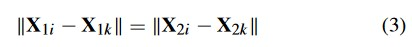
\includegraphics{eq3.jpg}
   \end{center}
By computing the object points using the matched image
points and (1) and comparing combinations of object point
pairs using (3), they form a subset that most likely contains
only inliers and use those for computing the translation
parameter T.\\
\section{Improved Feature Detection in Challenging
Environments}

Scale Invariant Feature Transform (SIFT) is an
approach based on transforming an image into local feature
vectors; SIFT descriptors, describing the intensities around
image points that are found as maxima or minima of a
difference-of-Gaussian function. Each vector is invariant to
image translation, scaling, and rotation and partially invariant
to illumination changes and affine or 3D projections. Due
to these invariances, SIFT provides good performance for
detecting distinctive features that may be matched across
images and therefore its improved variants have been developed, such as real-time detector FAST and SURF
that provide improved detection accuracy. However, these
detectors use Gaussian derivatives as smoothing kernels in
the detection process, which smooths relevant detail such as
object boundaries from the images, while removing noise.
When navigating in an initially feature-poor environment it
is essential to detect all features, even the weaker ones and
therefore even SURF fails frequently. Kaze is a feature
detector and descriptor based on nonlinear diffusion filtering.
Kaze provides multiscale features that have high repeatability
and distinctiveness. However, creating Kaze detectors and
descriptors takes approximately 2.5 times more computation
time than SURF and in the safety-critical applications requiring real-time processing Kaze cannot be the only solution.
Therefore, in the research the authors detect first SURF features and
then if that fails, look for Kaze features.
Figure 2.1 shows Kaze feature matching a detection result in
a feature poor corridor environment where not a single SURF
feature was found.
\begin{figure}
    \centering
    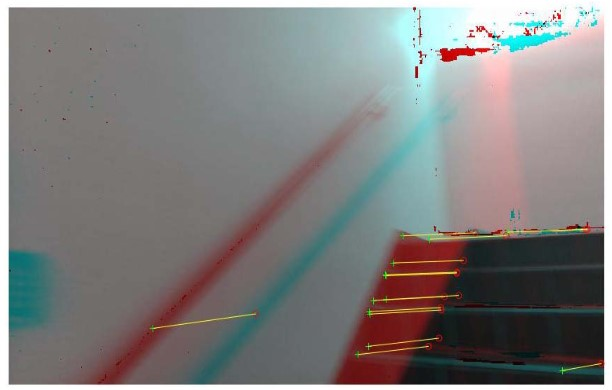
\includegraphics{f1.jpg}
    \caption{Kaze feature matching a detection result in
a feature poor corridor environment where not a single SURF
feature was found.}
    
\end{figure}

\section{Detecting Collaborators} 
Computation of a camera egomotion relies on tracking
features found from static objects. If the tracked features
are detected from dynamic objects, camera motion is accidentally fused with the object motion, resulting in erroneous
solution. However, the collaborative navigation setting by nature contains multiple moving pedestrians in the nearby
area. Therefore, it is essential to detect the pedestrians found
in images and remove their features from the tracked ones.
Figure 2.2 shows an example of the common problem; the
visual navigation method has detected SURF features and
matched them across two images for computing the camera
egomotion at the time interval between taking the images.
In this case, most of the features have been detected from a
dynamic pedestrian resulting in an erroneous visual odometry
solution. In recent years low-level feature detection models
based on Convolutional Neural Networks (CNN) have
achieved good performance. Development of methods
for detecting high-level features, has been accelerated by the
research focusing on autonomous traffic, where the detection
of for example pedestrians is crucial.\\
The appearance of humans in the images of a collaborative
navigation setting is complicated by many of the challenges
found in pedestrian detection, most likely even more than
in the largely addressed topic of detecting pedestrians from
vehicle cameras. These challenges arise from differences of
scale of humans in the images, their attitude, angle of view,
illumination changes and occlusion caused by other humans.
When in transport applications humans are usually detected
outdoors and with moderate distance between the camera and
the pedestrian, in indoor collaborative navigation the lighting
is challenging and close to each other and thereby the camera.
Occlusions arise, resulting in situations where specific body
parts are not visible, and a human should be detected from
non-human looking figures. Figure 2.3 shows a typical view
from a collaborative navigation situation.\\
\begin{figure}
    \centering
    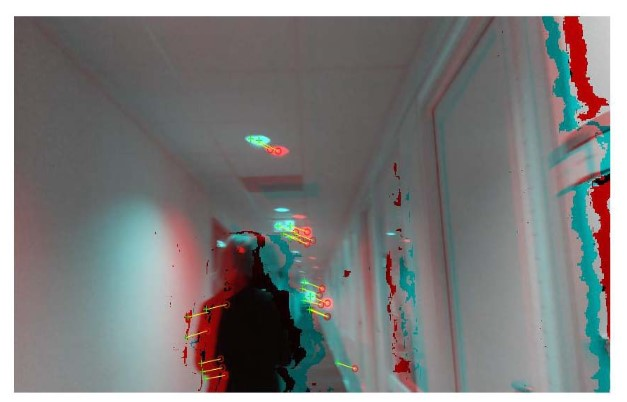
\includegraphics{f2.jpg}
    \caption{SURF features detected and matched (green crosses in image
1 and red circles in image 2.2) in an image from an indoor corridor. Majority
of the features are detected from a dynamic pedestrian.}
    
\end{figure}
YOLOs are
the cutting edge of the object detection. They usually use a
pre-trained CNN as basis for feature extraction. YOLOs split
the input image into a grid of cells and for each cell directly
predicts a bounding box locating an object if there is one inside
the box and simultaneously provide its classification.\\
\begin{figure}
    \centering
    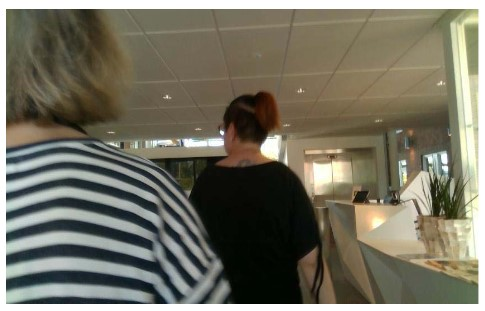
\includegraphics{fig3.jpg}
    \caption{Typical camera view in a collaborative navigation setting.}
    
\end{figure}
Here the authors have used a method based on YOLOv2 model
for detecting pedestrians in images in the collaborative navigation setup. Deficiency in YOLOv2 is that it is not able
to utilize effectively low-level features, and therefore detect
pedestrians that are at a long distance from the camera
appearing small in the images. However, this inability does
not degrade this navigation solution. Objects with a larger
distance than 10 meters from the camera are discarded due to
the RealSense depth detection limits and therefore, the presence of distant pedestrians is not disturbing the computation.
YOLOv2 object detection network is composed of two subnetworks. A feature extraction network followed by a detection
network. This YOLOv2 based implementation uses a pre-
trained ResNet-50 CNN as a backbone for feature extraction
and Activation40ReLU for detection trained using images
collected during various cooperative navigation experiments.
Before training the object detector with 1000 selected images,
they augmented the data to avoid over-fitting the model to
the data. In this case they are not increasing the number
of images in the data set, but warping them to increase
variability. Out of the 1000 manually labelled images they used
600 for training and the remaining 400 images for evaluation of the method. For optimization they used Stochastic Gradient
Descent with Momentum (SGDM) with mini-batch size 16 and
learning rate 0.001. They trained the model using 20 epochs.
When the batch size is 16 for 600 images, one epoch takes
38 iterations to complete, and thereby the number of iterations
for 20 epochs is 760.\\
Figure 2.4 shows the training loss for each iteration, Figure 2.5
the training root mean square error (RMSE) and Figure 2.6 precision (ratio of the detected pedestrians, ie. true positives, to all
instances that were inferred to be pedestrians) and recall (ratio
of detected pedestrians to all pedestrians in the data set) for the
training and learning processes. Average precision was 70\%,
which is in line with the accuracy of conventional pedestrian
detectors in challenging indoor lighting environments.
\begin{figure}
    \centering
    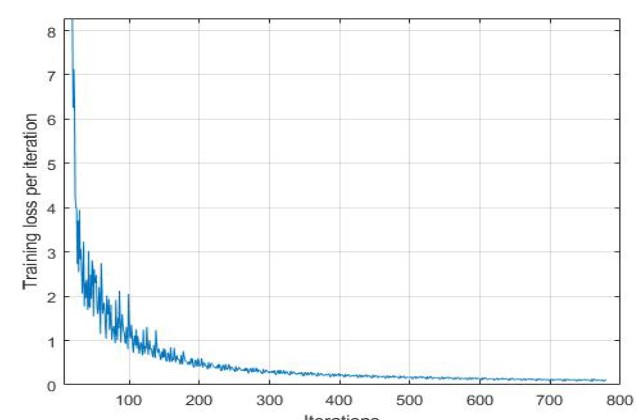
\includegraphics{f4.jpg}
    \caption{Training loss per iteration.}
    
\end{figure}
\begin{figure}
    \centering
    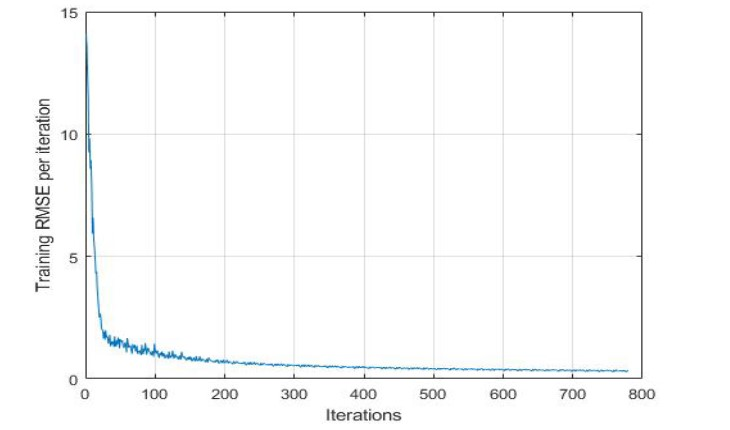
\includegraphics{f5.jpg}
    \caption{Training error per iteration.}
      
\end{figure}
\begin{figure}
    \centering
    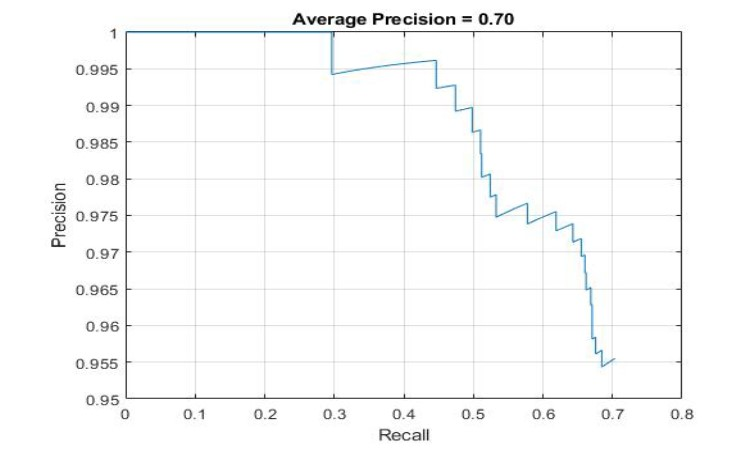
\includegraphics{f6.jpg}
    \caption{Precision and recall for pedestrian detection.}
    
\end{figure}
\section{Visual Odometry Solution} 

The final goal of the research is to first fuse tightly inertial
sensor measurements with visual odometry and then use
cooperative navigation for correcting the resulting individual
navigation solutions. Due to the challenging navigation environment and setup, the challenges degrading the visual odometry solution have to be understood and mitigated. Therefore,
the authors have computed a stand-alone visual odometry solution
using a RealSense D435 depth camera attached rigidly to the
user’s torso, and incorporated the improvements presented in
this section.\\
Image points were detected and matched from the images
using SURF features providing efficient computation, but
when there were too few points, Kaze features were detected.
Wrong matches were discraded using the RANSAC algorithm.
The presence of pedestrians in the image was detected using the YOLOv2 detector and the points inside the boxes were discarded. Also, points inside a 30 pixel wide area from the image
left side were discarded as non-reliable due to the RealSense
depth computation approach. RealSense D435 provides
the depth solution reliably only for objects closer than
10 meters from the camera. Unfortunately, the resulting depth
measurements are not consistent over an image in a dynamic
scenario and for objects further away from the camera. These
challenges affected mainly the speed solution of the visual
odometry and the attitude with lesser extent. The resulting
speed solution had random oscillation, which was filtered by
using a very basic Kalman filter.\\
Visual odometry (VO) requires at least five successfully
matched eligible image features when a calibrated camera is
used for computing the relative camera pose and four points to
get the pose into the orientation and translation with respect
to the world coordinates. The VO solution uses 3D to 2D
Perspective-n-Point (PnP) algorithm for computing the camera
pose. Bucketing is generally used in computer vision
research for computing the VO solution. The benefits
of using bucketing are reducing the number of features for
decreasing computational complexity of the algorithm as well
as guaranteeing good distribution of the image points through
the image. However, in our use case the challenge is the
scarcity of feature points, so neither of the benefits would be
achieved and therefore bucketing is not used. The VO solution
would be improved using a method called keyframing.
Keyframing means that feature correspondences are not only
computed to two consecutive images, but to a number of
previous images, keyframes making the pose estimation more
robust. The goal of this paper was to address the challenges due to monocular depth ambiguity, moving objects and
scarcity of features, therefore keyframing will be left for future
research.\\
The navigation setup includes multiple areas, where less
image points than required by VO are detected in total, such
as indoor staircases, or areas where all detected features are
farther than five meters from the user and thereby must
be discarded due to an erroneous depth solution. In these
situations the computation is evaluated to have failed and
such epochs are excluded from navigation. Figure 2.7 shows
the flow-chart of the visual odometry processing. \\
\begin{figure}
    \centering
    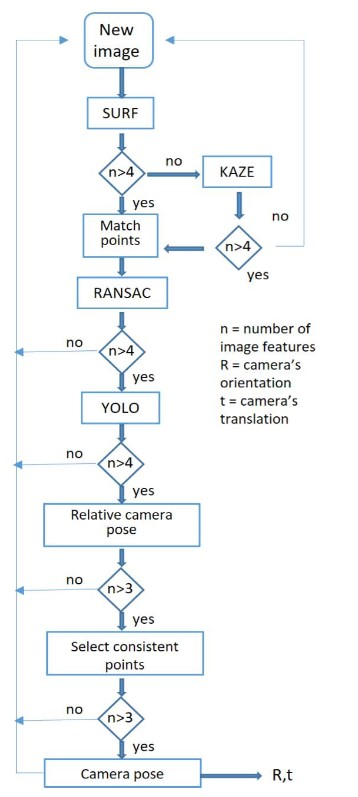
\includegraphics{fig7.jpg}
    \caption{Flowchart of the visual odometry process.}
    
\end{figure}
As the
VO solution is lost frequently due to these challenges, using conventional frame-to-frame methods, such as keyframing,
would not have been robust enough. Therefore, the authors have used
the basic Kalman filter mentioned before. The Kalman filter
state x consisted of only the horizontal speed s, x=\begin{math} s\end{math} filtering
out only large changes in the speed solution due to erroneous
VO observations. This setup resulted in very simple Kalman
filtering implementation, namely state-transition matrix A = 1,
covariance of the process noise Q = 0.001. The covariance of
the observation noise (R) was adapted to the error detection
in the observations described earlier. When the VO solution
was evaluated accurate R = 0.05, and when unreliable R was
set to R = 0.5.\\


